\chapter{K-indukciós algoritmus szoftverellenőrzésre}

Ebben a fejezetben bemutatom azokat a technológiákat, melyek szükségesek a programom algoritmikus részének a megértéséhez. Először kitérek a Control Flow Automata modellezés részleteire (Alfejezet \ref{sec:control_flow_automata}), aztán az előző fejezetben bemutatott jelölésrendszerrel formalizálom és ismertetem az algoritmust (Alfejezet \ref{sec:formalizalt_alg}).

\section{Control Flow Automata}
\label{sec:control_flow_automata}

A programokat sokféleképpen ábrázolhatjuk \cite{soft_ver_akos}. Legismertebb a programkód, melyet az ember könnyen, gyorsan tud írni olvasni, szemben a bájtkóddal, melyet a számítógép tud jóval hatékonyabban kezelni. A szoftveres modellellenőrzés elvégzéséhez a programkódot matematikailag pontos, formális ábrázolásban kell megadni, melyet a számítógép is jól tud használni. Egy széleskörűen ismert és használt ábrázolásmód a \emph{Control Flow Automaton} (CFA), mely egy gráf alapú ábrázolást biztosít a programokhoz. 

\paragraph{Szintaxis.}
A CFA  formálisan egy $\mathit{CFA} = (V, H, I_0, E)$ négyes \cite{beyer13}, ahol

\begin{itemize}
	\item $V = \{v_1, v_2, \ldots\}$ a változók halmaza. Mindegyik $v_i \in V$ változó rendelkezik egy $D_{v_i}$ doménnel, mely megszabja, hogy $v_i$ milyen értékeket vehet fel,
	\item \emph{H} a helyek halmaza,
	\item $I_0 \in H$ a kezdőhelye a gráfnak, a program belépőpontját jelöli,
	\item $E \subseteq H \times U \times H$ az irányított élek halmaza, melyek helyeket kötnek össze és a változókra vonatkozó utasításokkal vannak felcímkézve.
\end{itemize}

\paragraph{Utasítások.}
Háromféle utasítást különböztettem meg a dolgozatomban: 

\begin{itemize}
	\item A \emph{hozzárendelés} utasítás a $v_i := \mathit{kif}$ összefüggéssel írható le. Azt jelöli, hogy a baloldali $v_i \in V$ változóhoz hozzárendeljük a jobb oldali kifejezést. Fontos, hogy a $\mathit{kif}$ kifejezésnek is ugyanolyan doménnel kell rendelkeznie, mint a $v_i$ változónak.
	
	\item A \emph{feltevés} operátor a $[\mathit{cond}]$ formában írható le, ahol $\mathit{cond}$ egy bináris (\emph{Boolean}) kifejezés (feltétel). Ha egy él rendelkezik $\mathit{[cond]}$ feltétellel, akkor abban az esetben csakis akkor sülhet el (kerülünk át az egyik helyről a másikra), ha a feltétel teljesül. A feltétel egyik változóra sem hat ki, azok értékein nem változtat.
	
	\item A \emph{havoc} operátor a $\mathit{havoc}~v_i$ formában írható le, ahol $v_i \in V$ egy változó. A \emph{havoc} hozzárendel a $v_i$ változóhoz egy nem-determinisztikus értéket, a többi változót érintetlenül hagyja. Például arra lehet használni, mikor szimulálni szeretnénk a felhasználói bemenetet.
\end{itemize}
\ \\
Ha szeretnék egy olyan élet húzni két hely között, mely minden körülmények között elsül, akkor azt könnyen megtehetjük úgy, hogy nem adunk neki utasítást, vagy úgy is ha egy \texttt{[true]} feltételt adunk neki.

\paragraph{Grafikai megjelenítés.}
A helyeket körök, az éleket nyilak jelölik. Az egyes élek felett illetve mellett láthatóak az utasítások, amely jelen esetben hozzárendelés vagy feltevés. A kezdőállapotot egy bejövő nyíllal jelöljük. \cite{soft_ver_akos}.

\begin{example}
	Egy C nyelvű program és egy hozzátartozó CFA látható a (\ref{fig:cfa}) ábrán. A kezdőhely a $h_0$, a termináló hely a $h_7$, mely lehet végső- (final location) illetve hibahely (error location). Egy útvonal a kezdőhelytől a $h_4$ helyre leírható úgy, hogy $h_0 \rightarrow h_1 \rightarrow h_2 \rightarrow h_4$. A $h_1$ helyen egy elágazást figyelhetünk meg, ahol ha a $[y \leq 10]$ feltétel teljesül, akkor úgy a program a $h_1$ helyről továbbmegy a $h_2$ helyre, míg ha nem teljesül, akkor a $h_3$ helyre kerül a vezérlés. Az elágazásokban a kimenő élekre a feltételek úgy vannak megfogalmazva, hogy míg az egyiken az eredeti feltétel, addig a másikon annak a negáltja figyelhető meg. Ez azért van így, hogy szemléltesse az ábra, hogy ezt algoritmusok fogják feldolgozni, melyeknek könnyebb az egymást kizáró feltételek vizsgálata ebben a formátumban.
\end{example}

\begin{figure}[!htb]
	\begin{subfigure}[b]{.30\linewidth}
		\begin{lstlisting}
	int x = 1;
	if (y <= 10) {
			y = 10;
	} else {
			while (x < y) {
					x = 2 * x;
					y = y - 1;
			}
	}
	x = y + 1; \end{lstlisting}
	\caption{Egyszerű C program.}
	\label{fig:cfa1}		
	\end{subfigure}	
\hfill
\begin{subfigure}[b]{.63\linewidth}
	\centering
	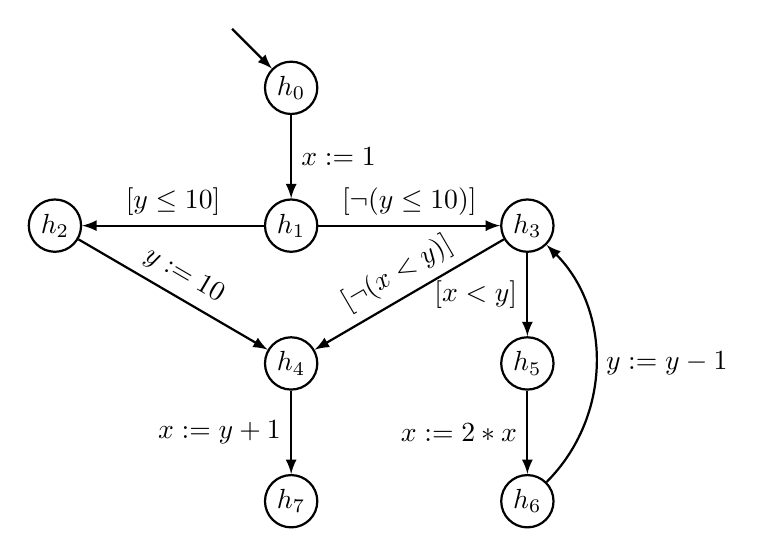
\begin{tikzpicture}
		\tikzstyle{loc}=[circle,align=center,draw,fill=white,thick,minimum size=0.6cm,inner sep=2]
		\tikzstyle{edge}=[-latex,thick]
		
		\node [loc] (l0) at (0, 0) {$h_0$};
		\draw[edge] (-0.75, 0.75)--(l0);
		
		\node [loc] (l1) at ( 0, -1.75) {$h_1$};
		\node [loc] (l2) at (-3, -1.75) {$h_2$};
		\node [loc] (l3) at ( 3, -1.75) {$h_3$};
		\node [loc] (l4) at ( 0, -3.5)  {$h_4$};
		\node [loc] (l5) at ( 3, -3.5)  {$h_5$};
		\node [loc] (l6) at ( 3, -5.25) {$h_6$};
		\node [loc] (l7) at ( 0, -5.25) {$h_7$};
		
		\draw[edge] (l0) -- node[midway, right]{$x := 1$}  (l1);
		\draw[edge] (l1) -- node[midway, above, sloped]{$[y \leq 10]$}  (l2);
		\draw[edge] (l1) -- node[midway, above, sloped]{$[\neg(y \leq 10)]$}  (l3);
		\draw[edge] (l2) -- node[midway, above, sloped]{$y := 10$}  (l4);
		\draw[edge] (l3) -- node[midway, above, sloped]{$[\neg(x < y)]$}  (l4);
		\draw[edge] (l3) -- node[midway, left]{$[x < y]$}  (l5);
		\draw[edge] (l4) -- node[midway, left]{$x := y+1$} (l7);
		\draw[edge] (l5) -- node[midway, left]{$x := 2*x$} (l6);
		\draw[edge] (l6) to [bend right = 45] node[midway, right]{$y := y-1$} (l3);
	\end{tikzpicture}
	\caption{A program CFA ábrázolása.}
	\label{fig:cfa2}
\end{subfigure}
\caption{Egy C program és a hozzátartozó Control Flow Automaton (CFA).}
\label{fig:cfa}
\end{figure}

\paragraph{Programábrázolás.} A (\ref{fig:structprog}) ábra megmutatja, hogy az alap elemei a strukturált programozásnak miként képezhetőek le CFA alakba \cite{soft_ver_akos}.
\begin{itemize}
	\item \emph{Szekvenciális} állításokat (\ref{fig:structprogseq} és \ref{fig:structprogseqcfa} ábra) úttal reprezentáljuk, mely helyek és élek közt alternál.
	
	\item \emph{Feltételes elágazásokat} (pl. \textit{ha-akkor} állítások, \ref{fig:structprogsel} és \ref{fig:structprogselcfa} ábra) különváló utakkal tudjuk reprezentálni őrfeltételekkel.
	
	\item \emph{Feltételes ciklusokat} (\ref{fig:structprogrep} és \ref{fig:structprogrepcfa} ábra) a CFA-ban körökkel tudunk ábrázolni. Egy vezérlési hely felel a ciklusfejért, amelyből két kimenő él fut. Az egyik bemegy a ciklusba, a másik pedig kilép abból. A ciklusban további szekvenciák, elágazások vagy akár újabb ciklusok is lehetnek, azonban az út mindig visszatér a ciklusfejhez.
\end{itemize}
\begin{figure}[!htb]
	\begin{subfigure}[b]{.29\linewidth}
		\begin{lstlisting}
			stmt1;
			stmt2;
			...\end{lstlisting}
		\caption{Szekvencia a programban.}
		\label{fig:structprogseq}		
	\end{subfigure}	
	\hfill
	\begin{subfigure}[b]{.29\linewidth}
		\begin{lstlisting}
			if (cond) {
				stmt1;
				...
			} else {
				stmt2;
				...
			}\end{lstlisting}
		\caption{Feltételes elágazás a programban.}
		\label{fig:structprogsel}		
	\end{subfigure}	
	\hfill
	\begin{subfigure}[b]{.29\linewidth}
		\begin{lstlisting}
			while (cond) {
				stmt;
				...
			}\end{lstlisting}
		\caption{Feltételes ciklus a programban.}
		\label{fig:structprogrep}		
	\end{subfigure}	
	\hfill
	\begin{subfigure}[b]{.3\linewidth}
		\centering
		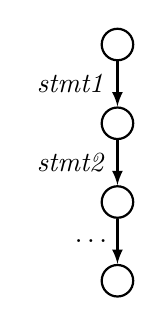
\begin{tikzpicture}
			\tikzstyle{loc}=[circle,draw,fill=white,thick,minimum size=0.4cm,inner sep=0]
			\tikzstyle{edge}=[-latex,thick]
			
			\node [loc] (l0) at ( 0, 0) {};
			\node [loc] (l1) at ( 0,-1) {};
			\node [loc] (l2) at ( 0,-2) {};
			\node [loc] (l3) at ( 0,-3) {};
			
			\draw[edge] (l0)--node[left]{$\mathit{stmt1}$}(l1);
			\draw[edge] (l1)--node[left]{$\mathit{stmt2}$}(l2);
			\draw[edge] (l2)--node[left]{$\ldots$}(l3);
		\end{tikzpicture}
		\caption{Szekvencia a CFA-ban.}
		\label{fig:structprogseqcfa}
	\end{subfigure}
	\hfill
	\begin{subfigure}[b]{.3\linewidth}
		\centering
		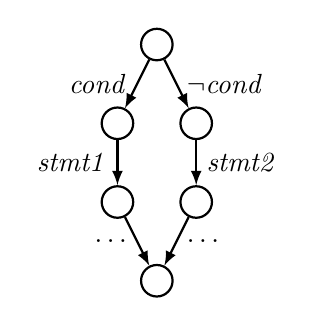
\begin{tikzpicture}
			\tikzstyle{loc}=[circle,draw,fill=white,thick,minimum size=0.4cm,inner sep=0]
			\tikzstyle{edge}=[-latex,thick]
			
			\node [loc] (l0) at (   0, 0) {};
			\node [loc] (l1) at (-0.5,-1) {};
			\node [loc] (l2) at ( 0.5,-1) {};
			\node [loc] (l3) at (-0.5,-2) {};
			\node [loc] (l4) at ( 0.5,-2) {};
			\node [loc] (l5) at (   0,-3) {};
			
			\draw[edge] (l0)--node[left]{$\assumeop{\mathit{cond}}$}(l1);
			\draw[edge] (l0)--node[right]{$\assumeop{\neg \mathit{cond}}$}(l2);
			\draw[edge] (l1)--node[left]{$\mathit{stmt1}$}(l3);
			\draw[edge] (l2)--node[right]{$\mathit{stmt2}$}(l4);
			\draw[edge] (l3)--node[left]{$\ldots$}(l5);
			\draw[edge] (l4)--node[right]{$\ldots$}(l5);
		\end{tikzpicture}
		\caption{Feltételes elágazás a CFA-ban.}
		\label{fig:structprogselcfa}
	\end{subfigure}
	\hfill
	\begin{subfigure}[b]{.3\linewidth}
		\centering
		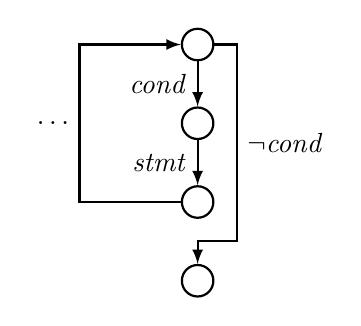
\begin{tikzpicture}
			\tikzstyle{loc}=[circle,draw,fill=white,thick,minimum size=0.4cm,inner sep=0]
			\tikzstyle{edge}=[-latex,thick]
			
			\node [loc] (l0) at ( 0, 0) {};
			\node [loc] (l1) at ( 0,-1) {};
			\node [loc] (l2) at ( 0,-2) {};
			\node [loc] (l3) at ( 0,-3) {};
			
			\draw[edge] (l0)--node[left]{$\assumeop{\mathit{cond}}$}(l1);
			\draw[edge] (l1)--node[left]{$\mathit{stmt}$}(l2);
			\draw[edge] (l2)--(-1.5,-2)--node[left]{$\ldots$}(-1.5,0)--(l0);
			\draw[edge] (l0)--(0.5,0)--node[right]{$\assumeop{\neg \mathit{cond}}$}(0.5,-2.5)--(0,-2.5)--(l3);
		\end{tikzpicture}
		\caption{Feltételes ciklus a CFA-ban.}
		\label{fig:structprogrepcfa}
	\end{subfigure}
	\caption{A strukturált programozás elemei (szekvencia, feltételes elágazás, feltételes ciklus) és a megvalósításuk CFA modelleken.}
	\label{fig:structprog}
\end{figure}

\subsection{Assert}
A verifikáció célja általában az, hogy a programban valamilyen tulajdonság teljesülését megcáfolja vagy bizonyítsa. Ehhez precízen meg kell fogalmaznunk, hogy pontosan milyen tulajdonságot szeretnénk ellenőrizni. Ezt megtehetjük az \emph{assert}-tel, mely azt ellenőrzi, hogy bizonyos változókon értelmezett feltétel teljesül-e. 
\newline
\newline
A CFA-ban az \emph{assert} egy speciális döntésként értelmezhető. Ha a feltétel igaz, a program a következő állapotnál folytatódik, ha pedig nem, akkor egy különálló $h_e \in H$ hibahelyre jutunk. Ha több ilyen \emph{assert} szerepel a programban, akkor a CFA hibahelyei összevonhatók: létrehozunk egy új hibahelyet, az összes többi hibahelyből vezetünk ide utasítás nélküli élet, majd a többi hibahelyet visszaminősítjük egyszerű vezérlési helynek. Az egyetlen megmaradt hibahely pedig egy, az Algoritmuselméletből\footnote{\url{http://www.cs.bme.hu/algel/}} jól ismert nyelőhely lesz. 

Vegyük észre, hogy a CFA megfelel egy, az előző fejezetben említett tranzakciós modellnek: vannak benne állapotok (helyek), melyek közt relációk húzódnak (élek). A kezdőhely az az állapot mely kielégíti a kezdőállapot tulajdonságot, illetve a hibahely az az állapot, mely nem teljesíti az assert-ben megfogalmazott feltételt a bejárás egy olyan pontján, ahol annak teljesítenie kéne.

Innentől kezdve az lesz a vizsgálatunk célja, hogy megállapítsuk, elérhető-e a hibahely az adott CFA-ban. Ezért a $(\mathit{CFA}, h_e)$ párost verifikációs feladatnak nevezzük -- a program \emph{helyes}, ha a hibahely nem elérhető, különben pedig \emph{hibás}.

\begin{example}
	Figyeljük meg a \ref{fig:assert1} ábrán az assert parancsot az ötödik programsorban. A programkódhoz tartozó CFA a \ref{fig:assert2} ábrán található, ahol a $h_3$ vezérlési helynél látható elágazás felel meg a program assert parancsának. Ha a feltétel teljesül, akkor a $h_f$ végső vezérlési helyre kerülünk és vége az ellenőrzésnek egy ``helyes'' kimenettel, míg ha nem teljesül a feltétel, akkor a $h_e$ hibahelyre jutunk és a verifikációs feladat egy ``hibás'' eredménnyel zárul, ekkor a program implementációján változtatni kell.
	\begin{figure}[!htb]
		\begin{subfigure}[b]{.43\linewidth}
			\begin{lstlisting}
			int x = 6;
			while (x > 0) {
						x--;
			}
			assert(x == 0);\end{lstlisting}
			\caption{C program \emph{assert} paranccsal.}
			\label{fig:assert1}		
		\end{subfigure}	
		\hfill
		\begin{subfigure}[b]{.56\linewidth}
			\centering
			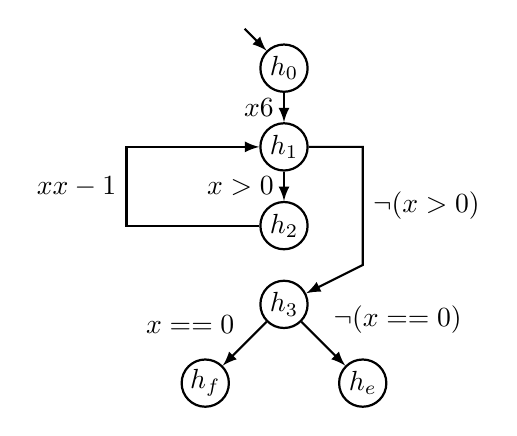
\begin{tikzpicture}
				\tikzstyle{loc}=[circle,draw,fill=white,thick,minimum size=0.6cm,inner sep=0]
				\tikzstyle{edge}=[-latex,thick]
				
				\node [loc] (l0) at (0, 0) {$h_0$};
				\draw[edge] (-0.5,0.5)--(l0);
				\node [loc] (l1) at (0,-1) {$h_1$};
				\node [loc] (l2) at (0,-2) {$h_2$};
				\node [loc] (l3) at (0,-3) {$h_3$};
				\node [loc] (lf) at (-1,-4) {$h_f$};
				\node [loc] (le) at (1,-4) {$h_e$};
				
				
				\draw[edge] (l0)--node[left]{$\assignop{x}{6}$}(l1);
				\draw[edge] (l1)--node[left]{$\assumeop{x > 0}$}(l2);
				\draw[edge] (l2)--(-2,-2)--node[left]{$\assignop{x}{x-1}$}(-2,-1)--(l1);
				\draw[edge] (l1)--(1,-1)--node[right]{$\assumeop{\neg (x > 0)}$}(1,-2.5)--(l3);
				\draw[edge] (l3)--node[above left]{$\assumeop{x == 0}$}(lf);
				\draw[edge] (l3)--node[above right]{$\assumeop{\neg (x == 0)}$}(le);
			\end{tikzpicture}
			\caption{A program CFA reprezentációja.}
			\label{fig:assert2}
		\end{subfigure}
		\caption{C program \emph{assert} paranccsal és a hozzátartozó CFA modell. A program \emph{assert} parancsát a CFA modell $h_3$ helye jelöli, mely hibás működés esetén a $h_e$ hibahelyre viszi a vezérlést.}
		\label{fig:assert}
	\end{figure}
\end{example}

\subsection{Állapottér}

A helyek ($ h_0, h_1, \ldots, h_n \in H $) a program futásának egyes állomásait jelölik, amik között a változók értékei változnak. Így nem tudjuk, hogy egy adott helyen például az egyes \textit{x}, \textit{y} változók értéke mennyi, mert azt a hely nem tárolja. Ezért bevezetjük az \textbf{állapot} fogalmát, mely két elemből fog állni: (1) az aktuális $ h \in H $ helyből illetve (2) a $ v \in V $ változók aktuális hozzárendelt értékeiből. Így, az összes lehetséges állapot \textit{A} megkapható úgy, hogy: $ A = L \times D_{v_1} \times \ldots \times D_{v_n} $. Az aktuális állapot a következő listából áll: $ (h, d_1, \ldots, d_n) \in A $, ahol $ h \in H $ az aktuális hely, $ d_i \in D_{v_i} $ pedig a $ v_i $ változóhoz hozzá rendelt értéke a $ D_{v_i} $ doménből.

Az algoritmusom csupán a helyek alkotta gráfot járja be és vizsgálja annak csúcspontjainak az elérhetőségét, az állapotokat (így a változók alakulását) nem veszi figyelembe. Ez azért van, mert már kevés hely és változó esetén is állapottér-robbanásról beszélhetünk, ugyanis az \textit{A} állapothalmaz mértékét a következőképp kaphatjuk meg: $ |A| = |H| \times |D_{v_1}| \times \ldots \times |D_{v_n}| $. Ami, ha nézünk egy kis példát, a következőképp alakul: vegyünk egy kis CFA-t 20 darab hellyel és 5 darab \texttt{int} változóval. Az \texttt{int} 4 byte-ton van tárolva, tehát a doménjének nagysága: $ D_{\mathit{int}} = 2^{32} $. Így az állapottér lehetséges mérete: $ |A| = 20 \times 2^{32} \times 2^{32} \times 2^{32} \times 2^{32} \times 2^{32} = 20 \times 2^{160} $. Az igaz, hogy a program nagy valószínűséggel ennek csak töredékét fogja a működése közben érinteni, viszont (1) ez nem ad garanciát arra, hogy valóban nem fogja bejárni illetve (2) ez még egy nagyon egyszerű CFA volt, egy korszerű biztonságkritikus rendszer nagyságrendekkel nagyobb.

Emiatt a programom ciklusmentes útvonalat nem tud vizsgálni, ugyanis ahhoz, hogy megállapítsuk a ciklusmentességet, az egyes helyekhez a változók értékeit is hozzá kell rendelni tehát az állapotokat kéne nézni. Felmerülhet, hogy miért nem elég csupán azt nézni, hogy hely ismétlődik-e az útvonalban. A helyek ismétlődhetnek az útvonalban, elég csak megnézni az előző (\ref{fig:assert}) ábrát: a helyes működés útvonalát a következőképp írhatjuk le: $ h_0 \rightarrow h_1 \rightarrow h_2 \rightarrow h_1 \rightarrow h_2 \rightarrow h_1 \rightarrow h_2 \rightarrow h_1 \rightarrow h_2 \rightarrow h_1 \rightarrow h_2 \rightarrow h_1 \rightarrow h_2 \rightarrow h_1 \rightarrow h_3 \rightarrow h_f $. Azért ismétlődhetnek, mert az helyes működésnek mondható, ha ugyanarra a helyre visszatérünk de más változó értékekkel. Azt viszont jó lenne kiszűrni, ha ugyanarra a helyre értünk vissza ugyanazokkal a változó hozzárendelésekkel, tehát ugyanarra az állapotra, mert ez esetben a modell bejárása közben végig egy végtelen ciklust is vizsgálni fog, amely a helyes működést nem befolyásolja, csak feleslegesen allokál CPU és memória-erőforrásokat.

\section{Az algoritmus formalizálása}
\label{sec:formalizalt_alg}

A dolgozatomban arra a kérdésre keresem a választ, hogy a (\ref{sec:problema_form})-es alfejezetben elmondottak segítségével hogy tudnánk belátni, hogy a modell a \emph{P} tulajdonságra nézve biztonságos?

Ezt például úgy tehetjük, hogy megnézzük tetszőleges nemnegatív \emph{i} egész esetén teljesül-e a
\begin{align}
	\label{eq:szimmetrikus}
	\forall s_{0} \dots s_{i}:~\neg(I(s_{0}) \wedge \mathit{utvonal}(s_{[0..i]}) \wedge \neg P(s_{i})),
\end{align}
feltétel. Ha megsérül valamelyik állapotban, akkor ezzel a módszerrel meg fogjuk találni és az oda vezető útvonal ellenpélda lesz a modell \emph{P}-biztonságosságára. Ez egy kívánatos eredmény: az algoritmusnak két féle kimenetele kell, hogy legyen: vagy az, hogy a modell \emph{P}-tulajdonságra nézve biztonságos (minden állapot teljesíti), vagy az, hogy a modell nem \emph{P}-biztonságos, ekkor egy ellenpéldát kell adnia, mely bizonyítja, hogy a  kezdőállapotból elindulva, azon végighaladva valóban egy hibaállapotba kerülünk.
\newline
\newline
Ha a rendszer \emph{P}-biztonságos, akkor (\ref{eq:szimmetrikus}) minden \emph{i}-re igaz lesz, hiszen nem fogunk tudni találni olyan \emph{i} értéket, melyre ne teljesülne. Felvetődhet a kérdés, hogy mikortól lehet azt mondani, hogy \emph{i} további növelése céltalan, mert már teljes bizonyossággal kijelenthetjük, hogy a modell \emph{P}-biztonságos? Az $I(s_{0}) \wedge \mathit{utvonal}(s_{[0..i]})$ feltétel önmagában nem fog gyorsítást eredményezni: végig megy az állapottéren amilyen hosszan csak lehetséges (ezt szeretnénk lerövidíteni), tekintve, hogy minden állapotnak van egy szülőállapota a \emph{T} tranzakciós reláción keresztül.
\newline
\newline
Ennél jobb stratégia, ha akkor állunk meg, mikor $I(s_{0}) \wedge  \mathit{cmUtvonal}(s_{[0..i]})$ ellentmondásos lesz. Ezt használva addig folytatjuk a keresést, míg az összes, ciklusmentes útvonalat be nem jártuk. Legrosszabb esetben ekkor is végigmegy a program a teljes állapottéren, viszont ha az állapottérben ciklikusság figyelhető meg, akkor azt a stratégia maximálisan kihasználja: átlagosan rövidebb (de bizonyosan nem hosszabb) útvonalakat fog bejárni, mint az $I(s_{0}) \wedge \mathit{utvonal}(s_{[0..i]})$.
\newline
\newline
Ehhez hasonlóan tehetjük azt is, hogy addig ellenőrzünk, amíg a $\mathit{cmUtvonal}(s_{[0..i]})~\wedge~\neg P(s_{i})$ nem lesz ellentmondásos: egy, a \emph{P} tulajdonságot sértő állapotból (hibaállapotból) kiindulva addig megyünk ciklusmentes útvonalakon visszafelé, míg be nem járjuk a teljes állapotteret (ez esetben kijelenthetjük, hogy a rendszer nem-\emph{P}-biztonságos), ellenben ha nem járunk be minden állapotot, akkor a rendszer \emph{P}-biztonságos. Ez azzal magyarázható, hogy ha a kezdőállapot nem elérhető a hibaállapotból (mert visszafele haladva útközben elakadunk), akkor kijelenthetjük, hogy a modell biztonságos.
\newline
\newline
A \emph{k}-indukció alapú szoftververifikáció az előbb elmondottakra épül. A módszer lényege, hogy elindulunk mind a kezdőállapotból, mind a hibaállapotból: míg az előbbiből előrefelé, addig az utóbbiból visszafelé. Kijelenthető, hogy a modell biztonságos, ha az előrefelé haladó keresés bejárta a teljes állapotteret (azaz minden állapotot bejártunk már \emph{első eset})\footnote{Természetesen ha közben hibaállapotba jutna, akkor a teljes modellellenőrzés megakadna, s így nem tudná bejárni a teljes állapotteret.}, illetve abban az esetben is, ha a hátrafelé haladó keresés megakad (\emph{második eset}).
\newline
\newline
A (\ref{sec:k_induction})-as fejezetben bemutatott, és így a módszer nevét adó \emph{k-indukció} abból adódik, hogy ha a modellt bejárjuk \emph{k} mélységig, és arra jutunk a fentebb említett metodika alapján, hogy a modell biztonságos, akkor kijelenthető, hogy $k+1$ mélységre is biztonságos lesz \cite{donaldson_cikk}, illetve mellé az is, hogy ezzel az indukciós lépést bizonyítottuk \cite{k_induction_article}, tehát kijelenthetjük, hogy a modell valóban biztonságos. Ha találunk ellenpéldát, akkor azzal a modell nem-biztonságosságát láttuk be.

\subsection{Elérhetőség vizsgálata}

\paragraph{Definíció.}
Egy $s_i \in S$ állapot elérhető az $s_j \in S$ állapotból, ha létezik olyan útvonal, melynek első állapota $s_j$, az utolsó állapota $s_i$, és beadva az út tranzakciós reláció listáját bejárási sorrendben egy Sat-megoldóba az ``igaz'' értékkel tér vissza.
\newline
\newline
Eddig a tranzakciós relációról úgy volt csak szó, mint egy, az állapotok közti éleket leíró halmaz. Ezt most kibővítjük -- a relációknak lehetnek állításai, melyek vagy leírnak egy utasítást ($x := x + 1$), vagy egy feltételt fogalmaznak meg ($x > 0$) vagy nem-determinisztikus értékadást képviselnek ($\mathit{havoc}$). Ahogy bejárjuk az utat az állapottérben a relációkon keresztül, abban a sorrendben egymás mellé fűzzük konjunkcióval a tranzakciókat, melyről a Sat-megoldó eldönti, hogy kielégíthető-e vagy sem.
,
\begin{example}
	Ha például az útvonalunk az $s_0 \xrightarrow[\text{}]{\text{$T_1(s_0, s_1)$}} s_1 \xrightarrow[\text{}]{\text{$T_2(s_1, s_2)$}} s_2 \xrightarrow[\text{}]{\text{$T_3(s_2, s_3)$}} s_3$, és azt szeretnénk megtudni, hogy $s_3$ elérhető-e, akkor azt a $\mathit{Sat}(T_0 \wedge T_1 \wedge T_2)$ kifejezéssel meghívott Sat-megoldó fogja nekünk eldönteni, mely bináris típusú válasszal tér vissza: ``igaz'' választ ad ha a kifejezés kielégíthető, különben ``nem'' választ. Vegyük észre, hogy a $\mathit{Sat}(\mathit{utvonal}(s_0, s_1, s_2))$ kifejezés megegyezik a $\mathit{Sat}(T_0 \wedge T_1 \wedge T_2)$ kifejezéssel a (\ref{eq:relacio_sor}) egyenlet miatt.
\end{example}
Feltételezzük, hogy a Sat-megoldó a tranzakciós reláció szekvencián kívül képes kezelni az egyes tulajdonságok teljesülését is. Így például a $\mathit{Sat}(I(s_0) \wedge \neg P(s_5))$ akkor lesz igaz, ha $s_0$ kezdőállapot \emph{és} $s_5$ nem elégíti ki a \emph{P} tulajdonságot.

\subsection{Algoritmus}

%\paragraph{Algoritmus.}
Tekintsük az (\ref{alg:1}) algoritmust, mely a kezdőállapotból indulva inkrementálisan járja be az állapotteret. Az első \emph{if} a \verb+3.+ sorban két feltételt ellenőriz, melyek egy diszjunkcióval vannak összekapcsolva:
\begin{itemize}
	\item Az első feltétel megfelel a fentebb említett \emph{első eset}nek: azt nézi, hogy az aktuális bejárási mélységben van-e olyan állapot, melyet nem látogattunk meg még a kezdőállapotból indulva \emph{és} elérhető. Ha van, akkor akkor a \emph{Sat($\ldots$)} visszatérési értéke ``igaz'' lesz, mely a negált hatására ``hamis''ra fordul és folytatjuk tovább az ellenőrzést.
	
	\item A második feltétel megfelel a fentebb említett \emph{második eset}nek. Azt vizsgálja, hogy ha az $s_e \in S$ hibaállapotból indulva eljutunk egy $s_{e+i} \in S$ állapotba, akkor az utóbbiból a hibaállapot felé visszaindulva kialakuló ciklusmentes útvonal kielégíthető-e. Ha igen, akkor folytatjuk tovább az ellenőrzést.
\end{itemize}
A második \emph{if} a \verb+6.+ sorban azt vizsgálja, hogy az állapot, melyben éppen vagyunk ($s_i$) az:
\begin{itemize}
	\item hibaállapot-e, illetve,
	\item a kezdőállapotból elindulva elérhető-e.
\end{itemize}
Ha elérhető és hibaállapot, a modellellenőrzés véget ért mert egy ellenpéldát találtunk, mellyel vissza is tér az algoritmus, ha nem, akkor az ellenőrzés folytatódik tovább és növeljük eggyel a bejárási mélységet.
\ \\
\ \\
\ \\
\begin{algorithm}[H]
\label{alg:1}

\SetAlgoLined
% \KwResult{}
i = 0 \\
\While{True}{
	\If{
		$\neg \mathit{Sat}(I(s_0) \wedge \mathit{cmUtvonal}(s_{[0..i]})) \vee \neg  \mathit{Sat}(\mathit{cmUtvonal}(s_{[e+i..e]}) \wedge \neg P(s_e))$
	}{
		return True
	}
	\If{
		$\mathit{Sat}(I(s_0)~\wedge~\mathit{utvonal}(s_{[0..i]})~\wedge~\neg P(s_i))$
	}{
		return $s_{[0..i]}$
	}
	i = i + 1
}
\caption{Checking if system is \emph{P}-safe}
\end{algorithm}

\begin{comment}
\paragraph{Állítás.} Tegyük fel, hogy az (\ref{alg:1})-es algoritmus ``True'' válasszal tért vissza. Ekkor a modell \emph{P}-biztonságos.
\\
\\
\textit{Bizonyítás:} Ha az algoritmus ``True'' válasszal tért vissza, akkor a \texttt{3.} sorban található feltételekből tudjuk, hogy a lehető legalacsonyabb értékű \textit{k}-ra igaz az, hogy a $\mathit{Sat}(I(s_0) \wedge \mathit{cmUtvonal}(s_{[0..k]}))$ és a $\mathit{Sat}(\mathit{cmUtvonal}(s_{[e+k..e]}) \wedge \neg P(s_e))$ közül legalább az egyiknek hamisnak kell lennie. A \texttt{6.} sor alapján tudjuk \cite{k_induction_article}, hogy $i < k$ esetén:
\begin{align}
	I(s_0) \wedge \mathit{utvonal}(s_{[0..i]}) \wedge \neg P(s_i)
\end{align}
ellentmondásos, hiszen ellenkező esetben igazra értékelődött volna ki és ellenpéldával tért volna vissza a program. Nyilvánvalóan következik ebből, hogy ciklusmentes útvonalra is ugyanúgy igaz ez:
\begin{align}
	\label{igeqkegy}
	I(s_0) \wedge \mathit{cmUtvonal}(s_{[0..i]}) \wedge \neg P(s_i))
\end{align}
hiszen ha nincs olyan útvonal, mely egy kezdőállapotot összekötne egy hibaállapottal, akkor ciklusmentes útvonal sem lesz.
\\
\\
Innentől azt kell már csak belátnunk, hogy $i \geq k$-re a (\ref{igeqkegy})-as egyenlet igaz. Tudjuk, hogy:
\begin{align}
	\begin{split}
		I(s_0) \wedge \mathit{cmUtvonal}(s_{[0..i]}) \wedge \neg P(s_i) \rightarrow \\
		I(s_0) \wedge \mathit{cmUtvonal}(s_{[0..k]}) \wedge \mathit{cmUtvonal}(s_{[k..i]}) \wedge \neg P(s_i)
	\end{split}
\end{align}
illetve
\begin{align}
	\begin{split}
		\mathit{cmUtvonal}(s_{[e+i..e]}) \wedge \neg P(s_e) \rightarrow \\
		I(s_0) \wedge \mathit{cmUtvonal}(s_{[e+i..e+k]}) \wedge \mathit{cmUtvonal}(s_{[e+k..e]}) \wedge \neg P(s_i)
	\end{split}
\end{align}
\end{comment}















